% vim:syntax=tex

In this section we describe how a topic model-based feature location
technique can use changesets.

\begin{figure*}
\centerline{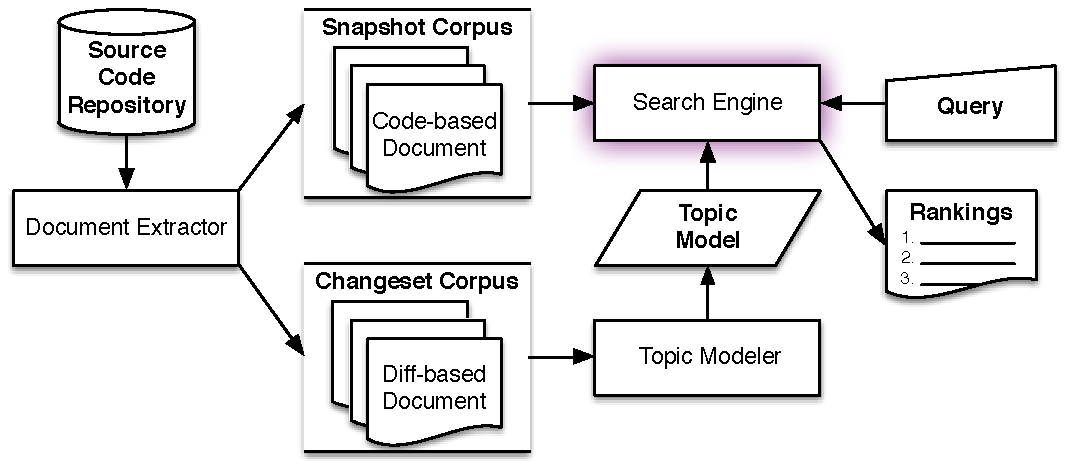
\includegraphics[width=.9\textwidth]{figures/changeset-flt}}
\caption{Feature location using changesets}
\label{fig:changeset}
\end{figure*}

In addition to the terminology described in Section~\ref{sec:related},
we use the following terminology to describe document extraction of changesets.
A \textit{diff} is a set of text which represents the differences between two texts.
A \textit{patch} is a set of instructions (i.e., diffs) that is used to transform one set of texts into another.
\textit{Context lines} denote text useful for transforming the text, but do not represent the differences.
\textit{Added lines} are lines which were added in order to transform the first text into the second.
Similarly, \textit{removed lines} are lines which are removed for this same purpose.
Figure~\ref{fig:diff} shows an example of what a changeset might look like.
A \textit{changeset}, ideally, represents a single feature modification,
addition, or deletion, which may crosscut many source code entities.
A \textit{commit} is a representation of a changeset in a version control system, such as Git or Subversion.

The changeset topic modeling approach requires two types of document extraction:
the snapshot of the state of source code at a commit of interest, such as a tagged release,
and every changeset in the source code history leading up to the same commit of interest.
The left side of Figure~\ref{fig:changeset} illustrates the dual-document extraction approach.

The document extraction process for the snapshot remains the same as covered in Section~\ref{sec:related} while the
document extractor for the changesets parses each changeset for the removed, added, and context lines.
The same preprocessor transformations as before occur in both the snapshots and changesets.
From there, each line is tokenized by the text extractor.
In a changeset it may be desirable to parse further for source code entities using island grammar parsing~\cite{Moonen:2001},
although not necessary for this approach.
It may also be desirable to only use portions of the changeset, such as only using added or removed lines.

The right side of Figure~\ref{fig:changeset} illustrates the retrieval process.
The key intuition to our approach is that a topic model such as LDA or LSI
can infer any given document's topic proportions regardless of the documents used to train the model.
Hence, we train a topic model on the changeset corpus and use the model to index the snapshot corpus.
Note that we never construct an index of the changeset documents on which the model is trained.

To leverage the online functionality of the topic models, we can also intermix the model training, indexing, and retrieval steps.
First, we initialize a model in online mode.
Then, as changes are made, the model is updated with the new changesets as they are committed.
That is, with changesets, we incrementally update a model and can query it at any moment.
Our temporal evaluation (\S~\ref{sec:methodology}) relies on this insight.

% In the search engine we can use a dynamic programming to keep the index up-to-date as new changesets are added to the model.
% That is, upon a update to the model, updates to the index are made only to the documents that are affected by the changesets.


\begin{figure*}[t]
\centering
\footnotesize
\begin{lstlisting}[language=diff, basicstyle=\ttfamily]
diff --git a/src/java/net/sf/jabref/EntryEditor.java b/src/java/net/sf/jabref/EntryEditor.java
index 8c56723..6b4788e 100644
--- a/src/java/net/sf/jabref/EntryEditor.java
+++ b/src/java/net/sf/jabref/EntryEditor.java
@@ -669,7 +669,8 @@ public class EntryEditor extends JPanel implements VetoableChangeListener {
     public void storeCurrentEdit() {
         Component comp = Globals.focusListener.getFocused();
         if ((comp == source) || ((comp instanceof FieldEditor) && this.isAncestorOf(comp))) {
-            ((FieldEditor)comp).clearAutoCompleteSuggestion();
+            if (comp instanceof FieldEditor)
+                ((FieldEditor)comp).clearAutoCompleteSuggestion();
             storeFieldAction.actionPerformed(new ActionEvent(comp, 0, ""));
         }
     }
\end{lstlisting}
\caption{Example of a \texttt{git diff}.
This changeset addresses JabRef's Issue \#2904968.
Black or blue lines denote metadata about the change useful for patching.
In particular, black lines represent context lines (beginning with a single space).
Red lines (beginning with a single~\texttt{-}) denote line removals,
and green lines (beginning with a single~\texttt{+}) denote line additions.}
\label{fig:diff}
\vspace{-10pt}
\end{figure*}
